\section{Experimentos e resultados}


\subsection{Experimentos}
Isso \'e o exemplo do experimento 1.

Ele consiste em analizar o tempo de converg\^encia entre a mudan\c{c}a de comunica\c{c}\~ao de n\'os entre o Soldado 2 e o Soldado 4.

\begin{figure}[H]
	\centering
	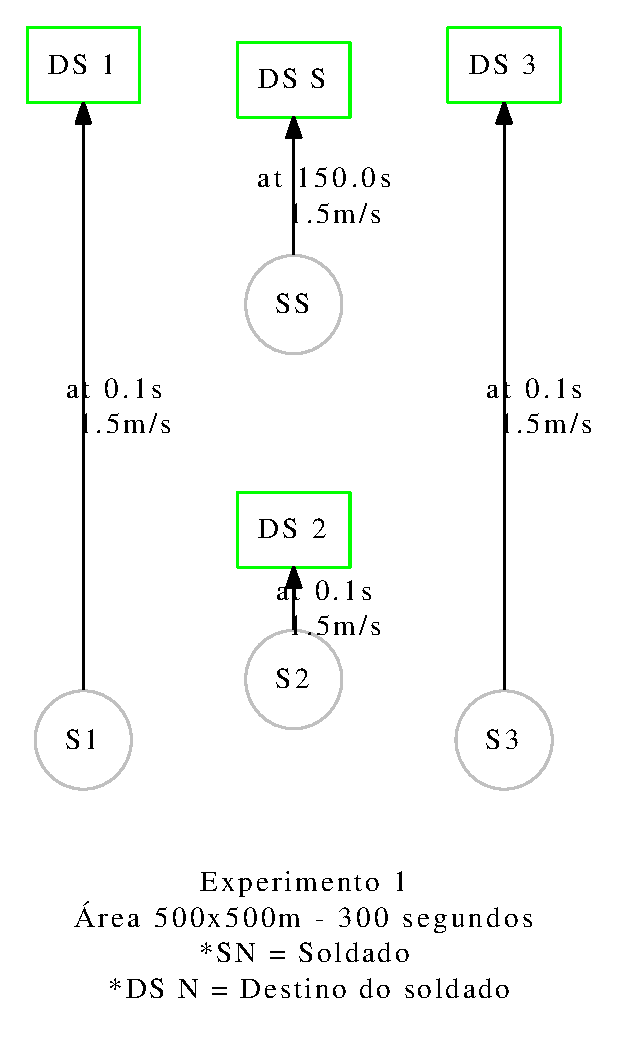
\includegraphics[scale=0.5]{experimento1.eps}
	\caption{Experimento 1}
	\label{figExp1}
\end{figure}

Isso \'e o exemplo do experimento 2.

Ele consiste em analizar o fuxo da rede passante.

\begin{figure}[H]
	\centering
	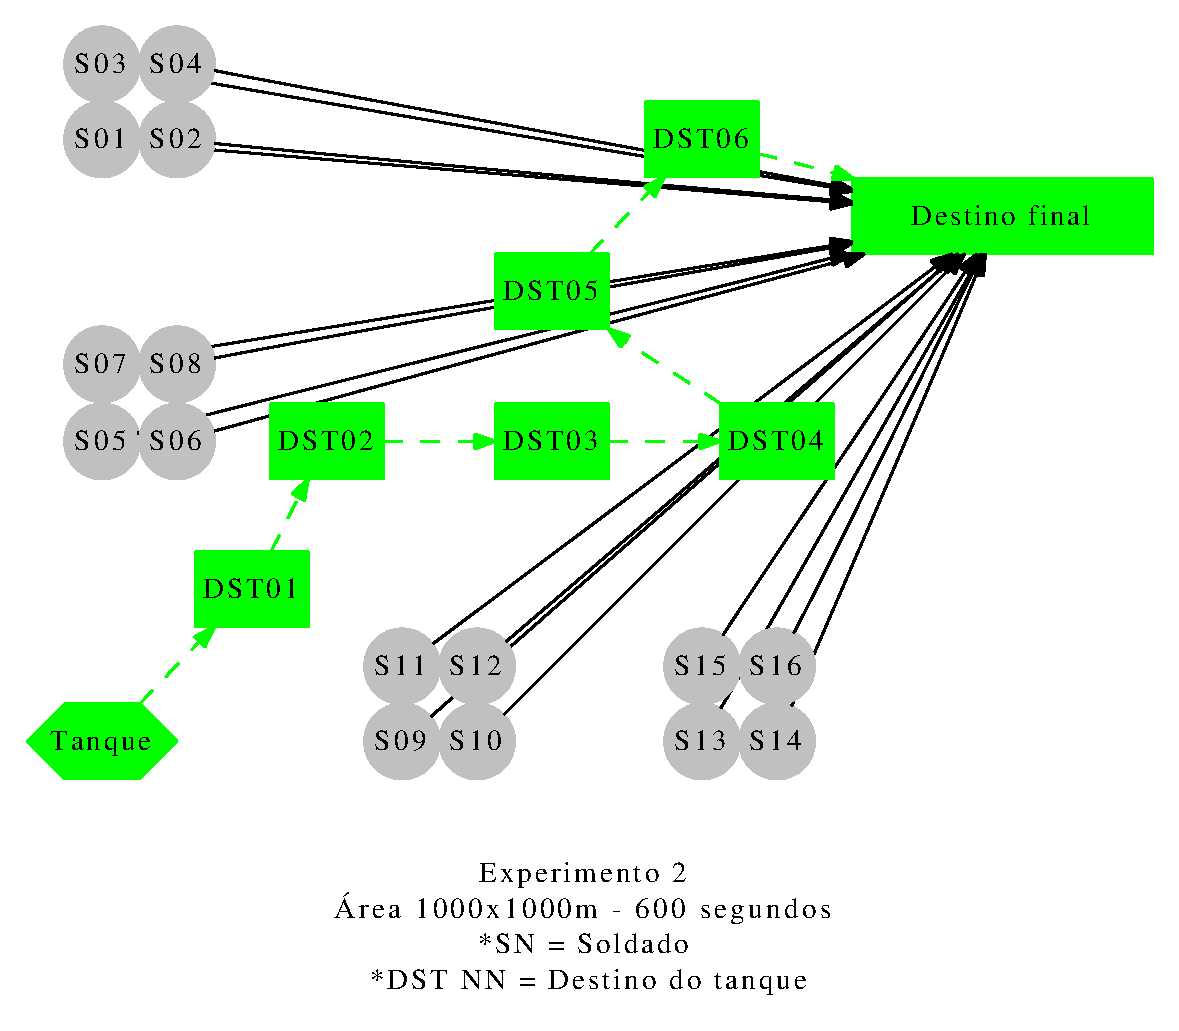
\includegraphics[scale=0.5]{experimento2.eps}
	\caption{Experimento 2}
	\label{figExp2}
\end{figure}


\subsection{M\'etricas de desempenho}
Baseando-se nos experimentos realizados por \cite{pereira} e nas informa\c{c}\~oes disponibilizadas por \cite{salles}, foram analizadas algumas m\'etrica a fim de comparar e concluir a oerformance de cada protocolos para cen\'arios militares.

As seguintes m\'etricas foram utilizadas:
\begin{itemize}
	\item taxa de entrega de pacotes
	\item atraso m\'edio fim a fim dos pacotes de dados
	\item n\'umero de pacotes de roteamento
	\item n\'umero de bytes de roteamento
\end{itemize}


\subsection{An\'alise comparativa dos resultados}

\begin{figure}[H]
	\centering
	\subfigure[Perda de pacotes]{
		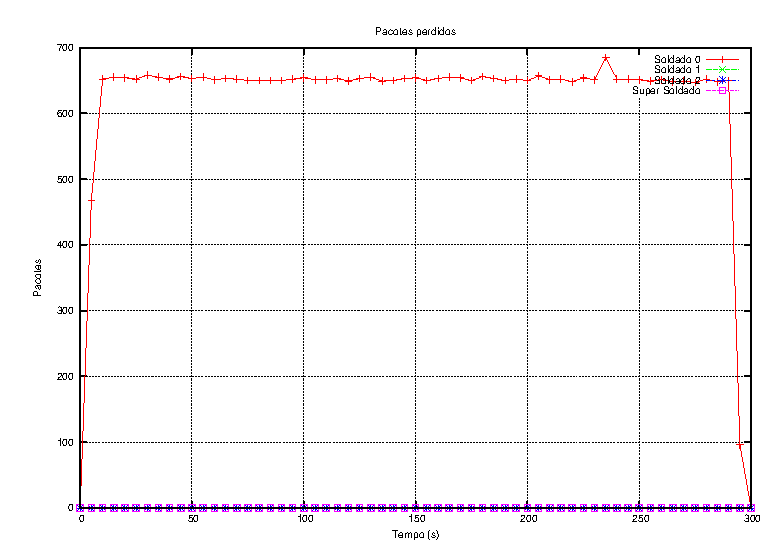
\includegraphics[scale=0.5]{aodvLost.eps}
	}\label{subfig:aodvLost}
	\subfigure[Atraso m\'edio (s)]{
		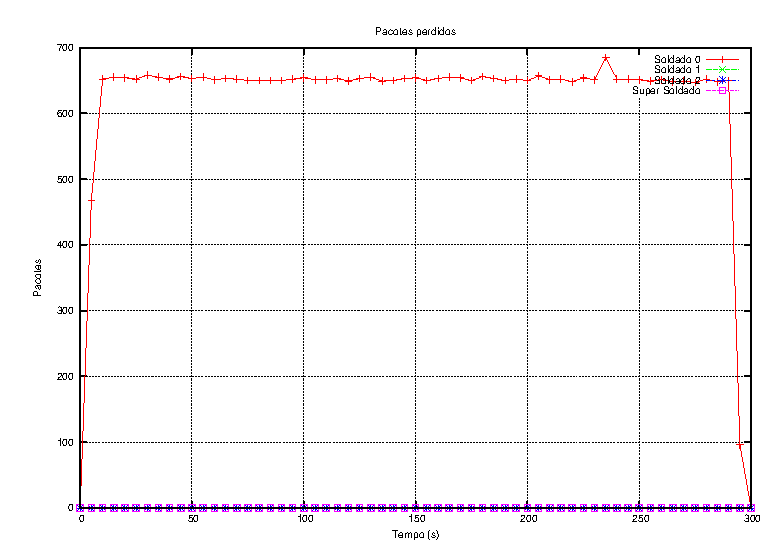
\includegraphics[scale=0.5]{aodvLate.eps}
	}\label{subfig:aodvLate}
	
	\caption{Resultados para o experimento 1}
	\label{fig:resulExp1}
\end{figure}

